\documentclass{article}
\usepackage[margin=1in]{geometry}
\usepackage{graphicx}
\usepackage[dvipsnames,table]{xcolor}
\usepackage[utf8]{inputenc}
\usepackage{siunitx}
\usepackage[american,siunitx]{circuitikz}
\usepackage{amsmath}
\usepackage{svg}
\usepackage{booktabs}
\usepackage{float}
\usepackage{xparse, xfp}
\usepackage{multirow}
\usepackage{tikz}
\usepackage{karnaugh-map}
\usepackage{pdfpages}
\usepackage{pdflscape}
\usepackage{hyperref}
\usepackage{adjustbox}
\usepackage[T1]{fontenc}
\usepackage{beramono}% monospaced font with bold variant
\usepackage{listings}
\lstdefinelanguage{VHDL}{  morekeywords={library,use,all,else,entity,if,elsif,then,others,is,or,port,in,out,end,process,architecture,of,    begin,and  ,LIBRARY,USE,ALL,ENTITY,IS,PORT,IN,OUT,END,ARCHITECTURE,OF, IF,ELSIF,THEN,   BEGIN,AND, PROCESS, CASE, DOWNTO, SIGNAL, COMPONENT, WHEN,OTHERS, TYPE,ELSE,WAIT,FOR,CONSTANT},  morecomment=[l]--}
\usepackage{xcolor}
\colorlet{keyword}{blue!100!black!80}
\colorlet{comment}{green!90!black!90}
\lstdefinestyle{vhdl}{  language     = VHDL,  basicstyle   = \ttfamily,  keywordstyle = \color{keyword}\bfseries,  commentstyle = \color{comment}}


\newcommand{\overbar}[1]{\mkern 1.5mu\overline{\mkern-1.5mu#1\mkern-1.5mu}\mkern 1.5mu}
\hypersetup{
    colorlinks=true,
    linkcolor=blue,
    filecolor=magenta,      
    urlcolor=cyan,
}
\usepackage{caption} 

\makeatletter
\ctikzset{lx/.code args={#1 and #2}{ 
  \pgfkeys{/tikz/circuitikz/bipole/label/name=\parbox{1cm}{\centering #1  \\ #2}}
    \ctikzsetvalof{bipole/label/unit}{}
    \ifpgf@circ@siunitx 
        \pgf@circ@handleSI{#2}
        \ifpgf@circ@siunitx@res 
            \edef\pgf@temp{\pgf@circ@handleSI@val}
            \pgfkeyslet{/tikz/circuitikz/bipole/label/name}{\pgf@temp}
            \edef\pgf@temp{\pgf@circ@handleSI@unit}
            \pgfkeyslet{/tikz/circuitikz/bipole/label/unit}{\pgf@temp}
        \else
        \fi
    \else
    \fi
}}

\ctikzset{lx^/.style args={#1 and #2}{ 
    lx=#2 and #1,
    \circuitikzbasekey/bipole/label/position=90 } 
}

\ctikzset{lx_/.style args={#1 and #2}{ 
    lx=#1 and #2,
    \circuitikzbasekey/bipole/label/position=-90 } 
}
\makeatother

\captionsetup[table]{skip=10pt}

\usetikzlibrary{calc, automata, positioning, decorations.markings}
%\usepackage[landscape]{geometry}
\renewcommand{\thesubsection}{\thesection.\alph{subsection}}
\newcommand{\equal}{=}
\newcommand{\greyrule}{\arrayrulecolor{black!30}\midrule\arrayrulecolor{black}}
\makeatletter
\newcommand\currcoor{\the\tikz@lastxsaved,\the\tikz@lastysaved}
\makeatother
\newcolumntype{:}{@{\hskip\tabcolsep\color{black!30}\vrule\hskip\tabcolsep}}

\ExplSyntaxOn
\NewExpandableDocumentCommand \groupify { O{\,\allowbreak} m m }
  { \jakob_groupify:nnn {#1} {#2} {#3} }
\cs_new:Npn \jakob_groupify:nnn #1 #2 #3
  { \__jakob_groupify_loop:nnw { 1 } {#2} #3 \q_recursion_tail {#1} \q_recursion_stop }
\cs_new:Npn \__jakob_groupify_loop:nnw #1 #2 #3
  {
    \quark_if_recursion_tail_stop:n {#3}
    \exp_not:n {#3}
    \int_compare:nNnTF {#1} = {#2}
      { \__jakob_groupify_sep:n }
      { \exp_args:Nf \__jakob_groupify_loop:nnw { \int_eval:n { #1+1 } } }
          {#2}
  }
\cs_new:Npn \__jakob_groupify_sep:n #1 #2 \q_recursion_tail #3
  {
    \tl_if_empty:nF {#2} { \exp_not:n {#3} }
    \__jakob_groupify_loop:nnw { 1 } {#1}
    #2 \q_recursion_tail {#3}
  }
\ExplSyntaxOff

\title{ECE 4300\\Discrete System Design Using VHDL\\\,\\Midterm 2}
 \author{Choi Tim Antony Yung (ID:013499993)}
\begin{document}
 \maketitle

% \thispagestyle{empty}
% \setcounter{page}{0}
 \newpage

\pagenumbering{gobble}

\section{Circuit from RTL Schematic}
The addition block and the increment block can be modeled with the + operator given that appropriate library be included and that the type is a vector. 
The multiplexer can be modeled with a case statement. The two registers can be modeled with a process block.
\subsection*{Code}
\subsubsection*{4x1 Multiplexer}
\lstinputlisting[style=VHDL]{ECE4304_Midterm2_VHDL/ECE4304_Midterm2_VHDL.srcs/sources_1/new/mux4x1.vhd}
\;\\
\subsubsection*{Main Circuit}
\lstinputlisting[style=VHDL]{ECE4304_Midterm2_VHDL/ECE4304_Midterm2_VHDL.srcs/sources_1/new/ECE4304_Midterm2_1.vhd}
\;\\
% \subsubsection*{Testbench}
% \lstinputlisting[style=VHDL]{ECE4304_Midterm1_VHDL/ECE4304_Midterm1_VHDL.srcs/sim_1/new/ECE4304_Midterm1_1_tb.vhd}
% \;\\
\newpage
\subsection*{RTL Schematic}
As can be seen in figure \ref{fig:1_RTL}, the RTL schematic resembles the given schematic.
\begin{figure}[H]
  \centering
  \caption{RTL Schematic of the Circuit}
  \includegraphics[width=\textwidth]{ECE4304_Midterm2_1_RTL.png}
  \label{fig:1_RTL}
\end{figure}

\newpage

\section{D Flip-Flop with Asynchronous Reset}
\subsection*{Code}
\subsubsection*{D Flip-Flop}
\lstinputlisting[style=VHDL]{ECE4304_Midterm2_VHDL/ECE4304_Midterm2_VHDL.srcs/sources_1/new/ECE4304_Midterm2_2.vhd}
\;\\
\subsection*{Schematic}
As can be seen in figure \ref{fig:2_sch}, the code models a D Flip-Flop with Asynchronous Reset.
\begin{figure}[H]
  \centering
  \caption{Schematic of the Circuit}
  \includegraphics[width=\textwidth]{ECE4304_Midterm2_2_sch.png}
  \label{fig:2_sch}
\end{figure}

\newpage

\section{}
\subsection{Assume $D_1 = 0$, $D_2 = 5$, and $D_1$ changes to 1 at time $= 10$ ns. What are the values of $D_1$ and $D_2$ after the following code has been executed once? Do the values of $D_1$ and $D_2$ swap?}
\begin{lstlisting}[style=VHDL]
RUN: process (D1)
begin 
    D2 <= D1; 
    D1 <= D2;   
end process;
\end{lstlisting}
Assuming it is synthesizable, as statements executes at the same time, when D1 change to be specific, D2 will get loaded with D1's value immediate at 10 ns and vice versa, D1 will be loaded 5 and D2 will be loaded 1.
In other words, it swaps after the process block was executed once.

\newpage
\subsection{Simplify the following code segment, i.e., what is it equivalent to?}
\begin{lstlisting}[style=VHDL]
process(a, b, c, d)
   begin 
   y <= a or c;
   y <= a and b;
   y <= c and d; 
end process;
\end{lstlisting}

It is equivalent to \lstinline[style=VHDL]{y <= c and d;}.\\

As only the last statement will be the final assignment to y,
it can be simplified to the following:
\begin{lstlisting}[style=VHDL]
  process(a, b, c, d)
     begin 
     y <= c and d; 
  end process;
  \end{lstlisting}

As change in a and b alone does not result in any change in y since it depend solely in c and d,
it can then be further simplified to the following:
\begin{lstlisting}[style=VHDL]
  process(c, d)
     begin 
     y <= c and d; 
  end process;
  \end{lstlisting}

As there is only one line inside the process and the sensitivity functionality of process block
is redundant with it consist of solely the signals which y is dependent on, the statement can be 
taken out of the process block while functioning exactly the same way, thus the final result:
\begin{lstlisting}[style=VHDL]
     y <= c and d; 
\end{lstlisting}

\newpage

\renewcommand\thesubsection{\thesection.\roman{subsection}}

\section{}

\begin{lstlisting}[style=VHDL]
  TST : process (clk, rst)
  begin
      if (rst = '1') then
          Q <= (others => '0');
      elsif (falling_edge(clk)) then
          if (CE = '1') then
              if (C = '0') then
                  Q <= A or B;
              else
                  Q <= A and B;
              end if;
          end if;
      end if;
  end process TST;
\end{lstlisting}

\subsection{Draw the circuit represented by the following Verilog process:}
The first three line inside the process block resembles the structure of a flipflop with asynchronous reset triggers
on falling edge. The nested if statements inside the \lstinline[style=VHDL]{elsif} block can then be modeled with multiplexer controlled with C going into another multiplexer controlled by CE going into D. 
As the \lstinline[style=VHDL]{else} of CE is not specified, it is assume that Q remain unchanged when CE = 0, meaning Q go into $X_0$ of mux controlled by CE.
From these information the following schematic can be constructed. Also, the \lstinline[style=VHDL]{Q <= (others => '0');} line
indicate that Q is a bus, thus A and B must also be bus as it would result in type mismatch otherwise.

\begin{figure}[H]
  \centering
\begin{circuitikz}[decoration={
  markings,
  mark= at position 0.5 with {\node[font=\footnotesize] {/};}
  }]
  \tikzset{flipflop custom/.style = {flipflop,
      flipflop def = {t1 = D, nd=1,c3 = 1, n3 = 1,t6 = Q, td = rst, nd = 0}
  }}
  \tikzset{mux 2x1/.style={muxdemux, muxdemux def={Lh=4, Rh=2, NL=5, NB=1, NR=1, w = 1.5}}}
  \draw
  (0,0) node[flipflop custom](DFF){}
  (DFF.pin 6) coordinate (Q) -- ++(0.5,0) node[right]{Q}
  (DFF.pin 1) coordinate (D)
  (DFF.pin 3) coordinate (CLK) node[left]{clk}
  (DFF.down) coordinate (RST) node[below]{rst}
  (D) -- ++(-1,0) node [mux 2x1, anchor = right, external pins width = 0](muxCE){} node[left] {\tiny{Y}}
  (muxCE.bottom) node[above]{\tiny{S}} -- ++(0,-0.5) node[below]{CE}
  (muxCE.lpin 2) node[right]{\tiny{$X_1$}} -- ++(-1,0) node [mux 2x1, anchor = right, external pins width = 0](muxC){} node[left] {\tiny{Y}}
  (muxC.bottom) node[above]{\tiny{S}} -- ++(0,-0.5) node[below]{C}
  (muxCE.lpin 4) node[right]{\tiny{$X_0$}} -- ++(-0.5,0) -- ++(0,-3) coordinate(tmp) -- (tmp-|Q) -- (Q)
  (muxC.lpin 2) node[right]{\tiny{$X_1$}} -- ++(-1,0) node[and port, anchor = out, scale = 0.7](and){}
  (muxC.lpin 4) node[right]{\tiny{$X_0$}} -- ++(-1,0) node[or port, anchor = out, scale = 0.7](or){}
  (and.in 2) -- ++(-0.5,0) -- (\currcoor|-or.in 2) node[circ](bx){} -- (or.in 2)
  (bx) -- ++(-1,0) node[left](B){B}
  (and.in 1) -- ++(-1,0) -- (\currcoor|-or.in 1) node[circ](ax){} -- (or.in 1)
  (ax) -- ++(-1,0) node[left](A){A}
  ;
  \path[postaction = {decorate}](DFF.bpin 1) -- (muxCE.right);
  \path[postaction = {decorate}](tmp) -- (tmp-|Q);
  \path[postaction = {decorate}](muxCE.blpin 2) -- (muxC.right);
  \path[postaction = {decorate}](muxC.blpin 2) -- (and.bout);
  \path[postaction = {decorate}](muxC.blpin 4) -- (or.bout);
  \path[postaction = {decorate}](bx) -- (B);
  \path[postaction = {decorate}](ax) -- (A);

\end{circuitikz}
\end{figure}

\subsection{Why rst is on the sensitivity list whereas C is not?}

As everything inside the elsif block happen only at the falling edge of the clock, 
the clk on the sensitivity already cover that block, thus no need to put C on sensitivity list.
However, since the reset is intended to be asynchronous, it cannot happen only when clk change,
thus the necessity to put rst on the sensitivity list such that reset can be trigger independent of the clock.

\section{Write the VHDL code that implements the graphical representation of the finite state machine (FSM) below using asynchronous modeling.}

\begin{figure}[H]
  \centering
  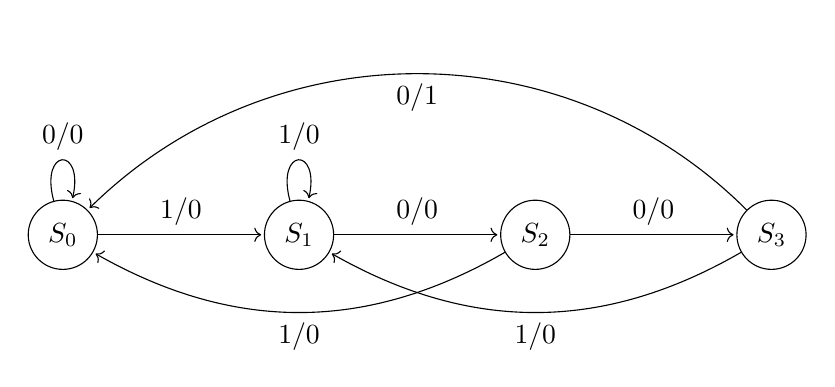
\begin{tikzpicture}[shorten >=1pt,node distance=3cm,on grid,auto] 
    \node[state] (s0)   {$S_0$}; 
    \node[state] (s1) [right =of s0] {$S_1$}; 
    \node[state] (s2) [right=of s1] {$S_2$}; 
    \node[state] (s3) [right=of s2] {$S_3$}; 
    \path[->]
     
    (s0) edge [loop above] node {0/0} ()
         edge node{1/0} (s1)
    (s1) edge [loop above] node {1/0} ()
         edge node{0/0} (s2)
    (s2) edge [bend left] node {1/0} (s0)
         edge node{0/0} (s3)
    (s3) edge [bend left] node {1/0} (s1)
         edge [bend right = 45] node {0/1} (s0)


     ;
  \end{tikzpicture}
\end{figure}

\subsection*{Code}
\lstinputlisting[style=VHDL]{ECE4304_Midterm2_VHDL/ECE4304_Midterm2_VHDL.srcs/sources_1/new/ECE4304_Midterm2_5.vhd}
\;\\
\subsection*{Testbench}
\lstinputlisting[style=VHDL]{ECE4304_Midterm2_VHDL/ECE4304_Midterm2_VHDL.srcs/sim_1/new/ECE4304_Midterm2_5_tb.vhd}
\;\\
\begin{figure}[H]
  \centering
  \caption{Simulation Waveform of the FSM}
  \includegraphics[width=\textwidth]{ECE4304_Midterm2_5_sim.png}
  \label{fig:5_sim}
\end{figure}
All 8 edges were tested:
\begin{itemize}
  \item 0/0, $S_0$ to $S_0$ at 15 ns
  \item 1/0, $S_0$ to $S_1$ at 25 ns
  \item 1/0, $S_1$ to $S_1$ at 35 ns
  \item 0/0, $S_1$ to $S_2$ at 45 ns
  \item 1/0, $S_2$ to $S_0$ at 55 ns
  \item 0/0, $S_2$ to $S_3$ at 85 ns
  \item 1/0, $S_3$ to $S_1$ at 95 ns
  \item 0/1, $S_3$ to $S_0$ at 125 ns
\end{itemize}

\end{document}
